The correctness of the leaf-level components introduced by CASE
transformations resolves to the question of whether such a component
meets its \agree{} contract. This proof obligation is approachable in
various ways: for example, it can be dealt with by inspection, unit
testing, or by formal proof. In CASE, we take a version of the formal
proof route: \emph{synthesis}. In particular, given a sufficiently
detailed formal contract, we generate code from it and generate proofs
showing that the generated code obeys the contract.

The formal languages that filters, gates, and monitors are generated
from include regular expressions, contiguity types
\cite{contiguity-types}, and Lustre\cite{lustre}. For each of these
languages, we have infrastructure (see Figure \ref{fig:synthesis})
that (a) translates formal specifications to code and (b) proves the
correctness of the translation. The generated code is CakeML
\cite{cakeml}, a verified compiler for a Standard ML variant.

\begin{figure}[h]
\begin{center}
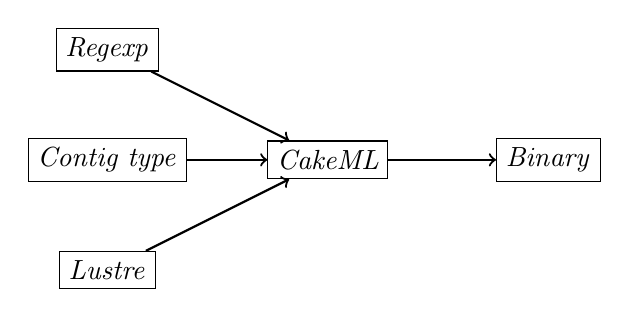
\begin{tikzpicture}[scale = 0.7]
\node (A) at (0,2) [shape=rectangle,draw]{\textit{Regexp}};
\node (B) at (0,0) [shape=rectangle,draw]{\textit{Contig type}};
\node (C) at (0,-2) [shape=rectangle,draw]{\textit{Lustre}};
\node (D) at (4,0) [shape=rectangle,draw]{\textit{CakeML}};
\node (E) at (8,0) [shape=rectangle,draw]{\textit{Binary}};
\draw [->,thick] (A) to (D);
\draw [->,thick] (B) to (D);
\draw [->,thick] (C) to (D);
\draw [->,thick] (D) to (E);
\end{tikzpicture}
\end{center}
\caption{Verified Synthesis Path.\label{fig:synthesis}}
\end{figure}

Regular expressions and contiguity types are well-suited for
expressing common data constraints used in determining the
wellformedness of messages in filters. Regular expressions compile to
efficient finite state automata; our regexp compiler has been proved
correct \cite{case-verified-filter}. Contiguity types capture more
complex data formats, including variable-length arrays and union
structures. We use a proved correct contiguity-type based parser
generator to decode serialized data and check wellformedness. A
Turing-complete language is required in order to support the
definition of gates and monitors, which can require arbitrarily
complex computations. Lustre, which underlies \agree{}, provides
that. We have formalized the semantics of Lustre and are using it as
the basis for a formal translation to CakeML. (Lustre is a
stream-oriented language which requires some interesting translation
steps in order to arrive at conventional code.)

Note that code generated from \splat{} is deployed as a scheduled
thread in a real-time environment. Thus there are two aspects to the
correctness of thread behavior: (1) correctness of a `one shot` thread
execution, as discussed above, and (2) correctness of the perpetual
thread execution. How to model the latter and prove relevant
properties is discussed in \cite{johannes:repeat}.
